\section{Hallazgos de la ampliación y controles}
En Taylor--Green gaussiano, TLS-DMD de rango cuatro pasa de 3.709\% a 1.684\% de error mediano de velocidad con proyección y banda declarada. En los tres casos newtonianos gaussianos, las condiciones aceptadas son 0 sin proyección y 12 con proyección. No se ajustó la banda utilizando la referencia limpia.
El dispatcher forward--backward a TLS utilizó su alternativa predeclarada en 23 condiciones. Los fallos primarios permanecen en los registros y su trabajo cuenta en el costo total.
\section{Pronóstico cronológico ejecutado}
Se evaluaron 60 condiciones con cinco campos, cuatro modelos de contaminación y tres semillas. Cada condición considera 29 opciones, con ajuste sólo en entrenamiento, selección por error de validación ruidosa y evaluación final en un bloque futuro independiente. Las opciones físicas comparten ajustes; no se cuentan como entrenamientos independientes.
La opción seleccionada mejora persistencia sin filtrar en 48 condiciones y persistencia filtrada en 43. Se exige una diferencia absoluta mayor que $10^{-10}$ en el error relativo de velocidad; las diferencias de redondeo se consideran empates. Estos conteos son condicionales al banco y no probabilidades de éxito en mediciones reales.
\begin{figure}[htbp]\centering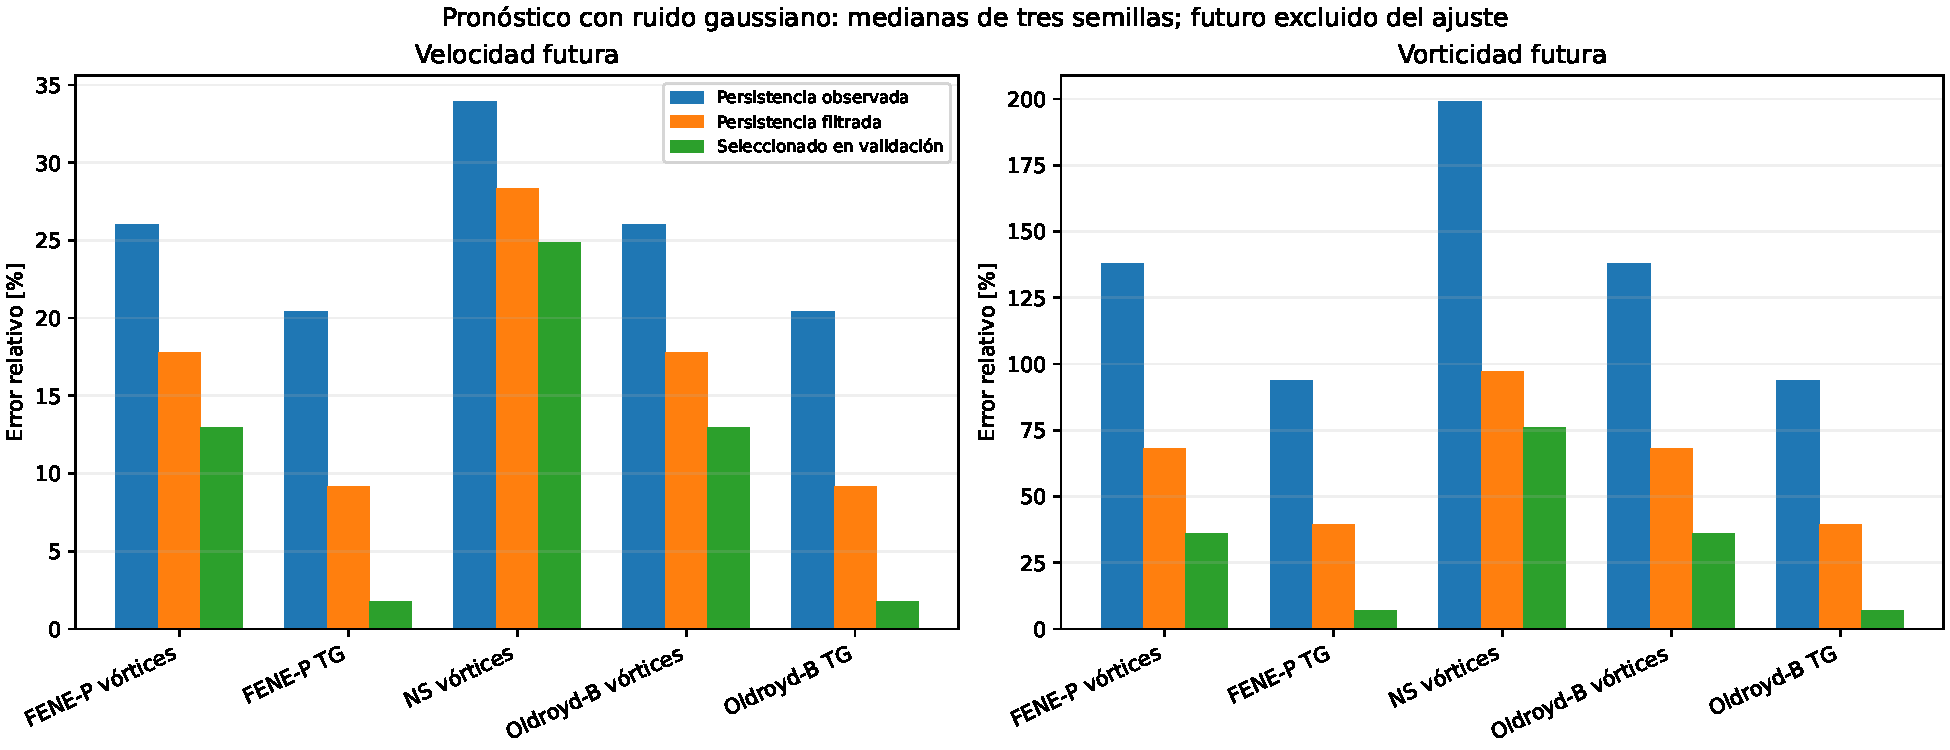
\includegraphics[width=\textwidth]{results/research/forecasting_extended_2026-10-14/figures/holdout_comparison.pdf}
\caption{Errores en el futuro excluido del ajuste. Comparar con persistencia filtrada evita atribuir toda mejora al modelo dinámico.}\end{figure}
\section{Banco reológico con condiciones iniciales comunes}
Seis fluidos comparten velocidad inicial, densidad, dominio, malla y tiempos. Las diferencias numéricas representan cambios constitutivos; no son errores de reconstrucción. Las viscosidades HB se igualan en la tasa de corte declarada y las constantes viscoelásticas se comparan en su normalización nominal. La cercanía Oldroyd-B/FENE-P observada no demuestra capacidad de identificar materiales con velocidad ruidosa.
\begin{figure}[htbp]\centering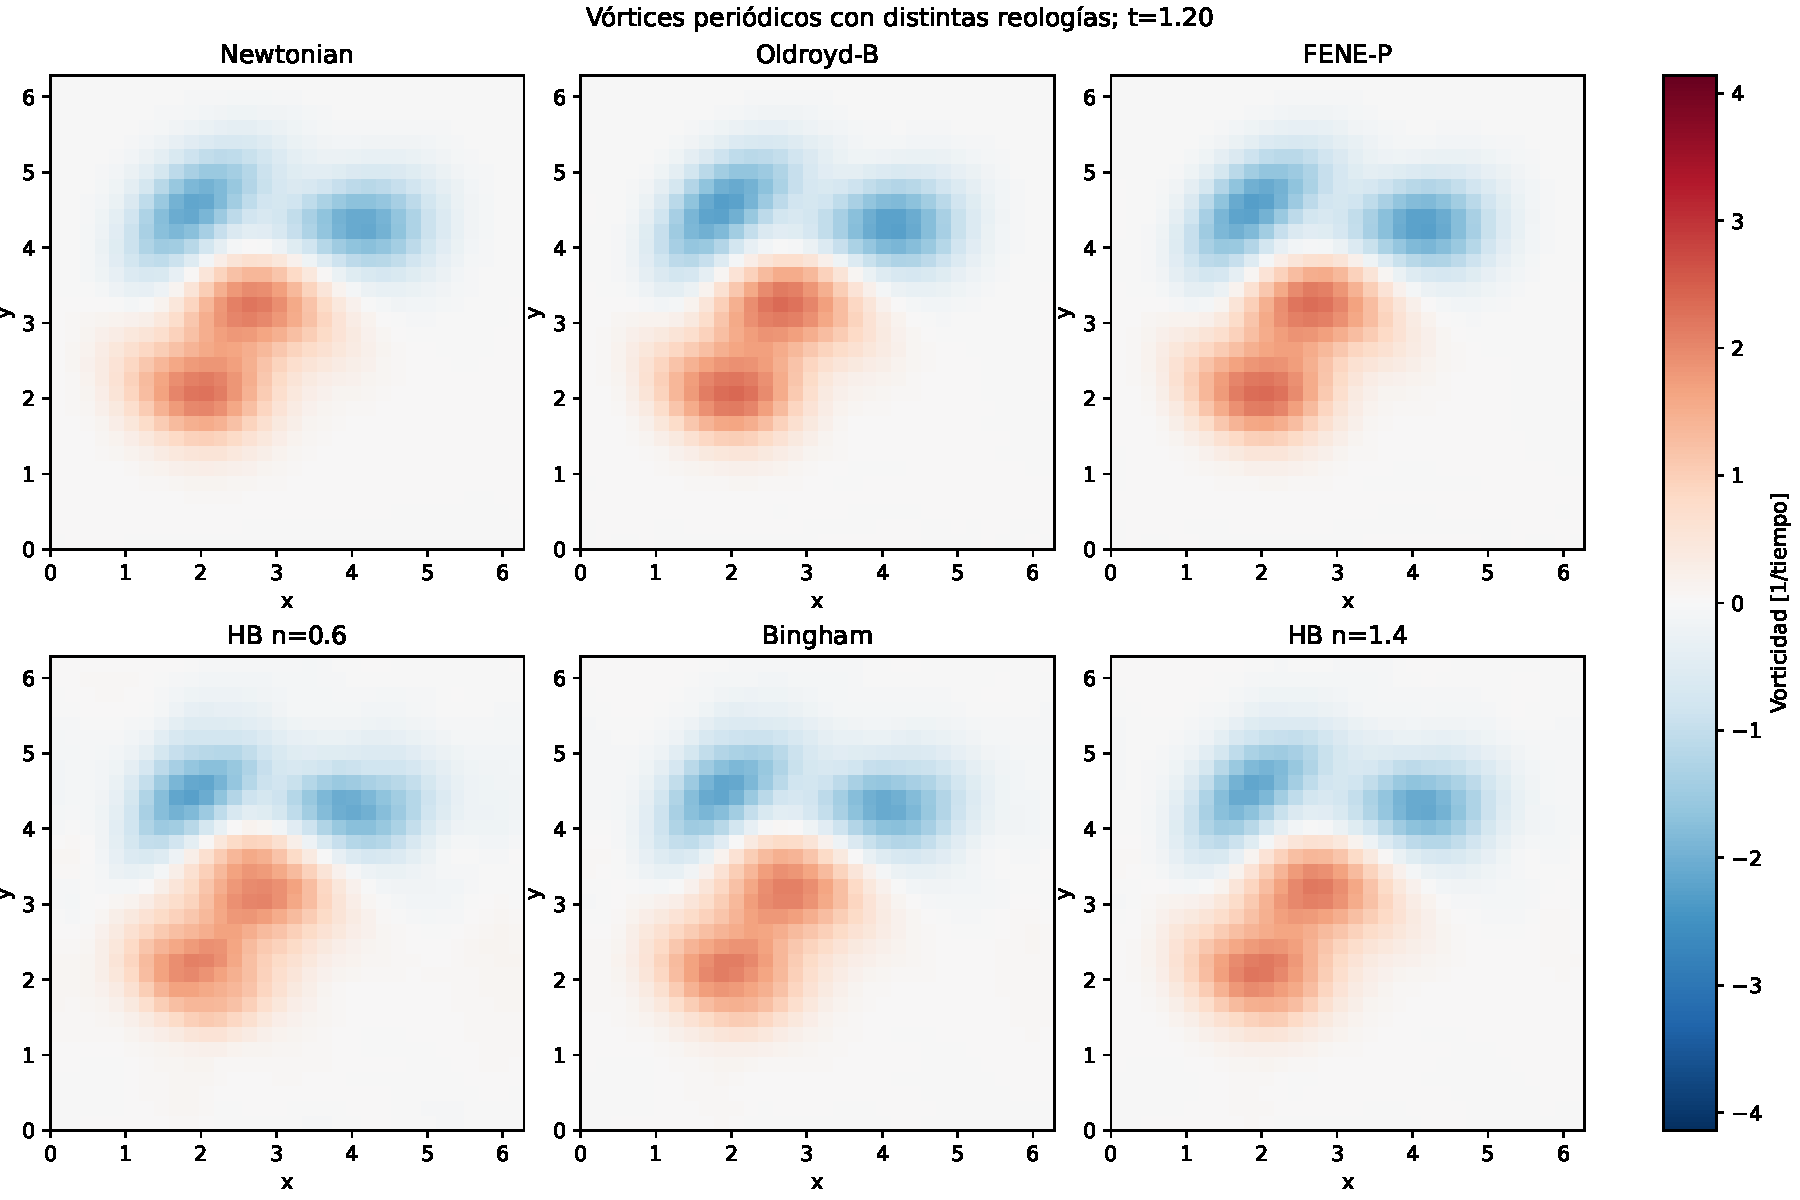
\includegraphics[width=\textwidth]{results/research/rheology_matched_2026-10-14/final_vorticity.pdf}
\caption{Vorticidad final de seis modelos sobre el mismo estado inicial periódico. Las diferencias dependen de la ley constitutiva y su normalización declarada.}\end{figure}
\section{Cuestiones todavía abiertas}
La vorticidad futura en casos de vórtices conserva errores importantes, y ninguna condición de ruido temporal o deriva de sensor satisface los umbrales de reconstrucción. La proyección reduce divergencia pero no recupera por sí sola sesgo de sensor, esfuerzos o memoria constitutiva. Los wakes externos, EVP, 3D, PIV, GPU y aprendizaje profundo siguen pendientes de ejecución.
